\documentclass[compress,professionalfont]{beamer}



\usepackage[latin1]{inputenc}
\usepackage{graphicx}
%\usepackage{pgf}

\usepackage{pstricks} 
\usepackage{pstricks-add} 
\usepackage{pst-plot} 
\usepackage{pst-text,pst-node,pst-tree} 

\usepackage{beamerthemeAmsterdam} 

%\hypersetup{pdfstartview={FitH}}


\setbeamertemplate{navigation symbols}{}
%\usetheme{Warsaw}
%\usecolortheme{beaver}
%\usefonttheme{structuresmallcapsserif}


\title[Point-Based Color Bleeding With Volumes]{PCBEX:\\Point-Based Color Bleeding With Volumes\\Thesis Defense}
\author{Christopher James Gibson}
\institute{California Polytechnic University\\CSC Department}
\date{June 9, 2011}

\setcounter{tocdepth}{1}

\begin{document}

\AtBeginSection[]
{
  \begin{frame}<beamer>
    \frametitle{Outline}
    \tableofcontents[currentsection,currentsubsection]
  \end{frame}
}




%%----------------------------------------------------------------------  TITLE
\begin{frame}

    \titlepage

\end{frame}




%%-------------------------------------------------------------------  SCHEDULE
\begin{frame}{Schedule}

\tableofcontents

\end{frame}




\section{Introduction}
%%---------------------------------------------------------------  INTRODUCTION
\begin{frame}{Graphics Intro}

    \begin{columns}
        \begin{column}{0.65\textwidth}
            Definition of graphics\\
            Graphics and light\\
        \end{column}
        \begin{column}{0.35\textwidth}
            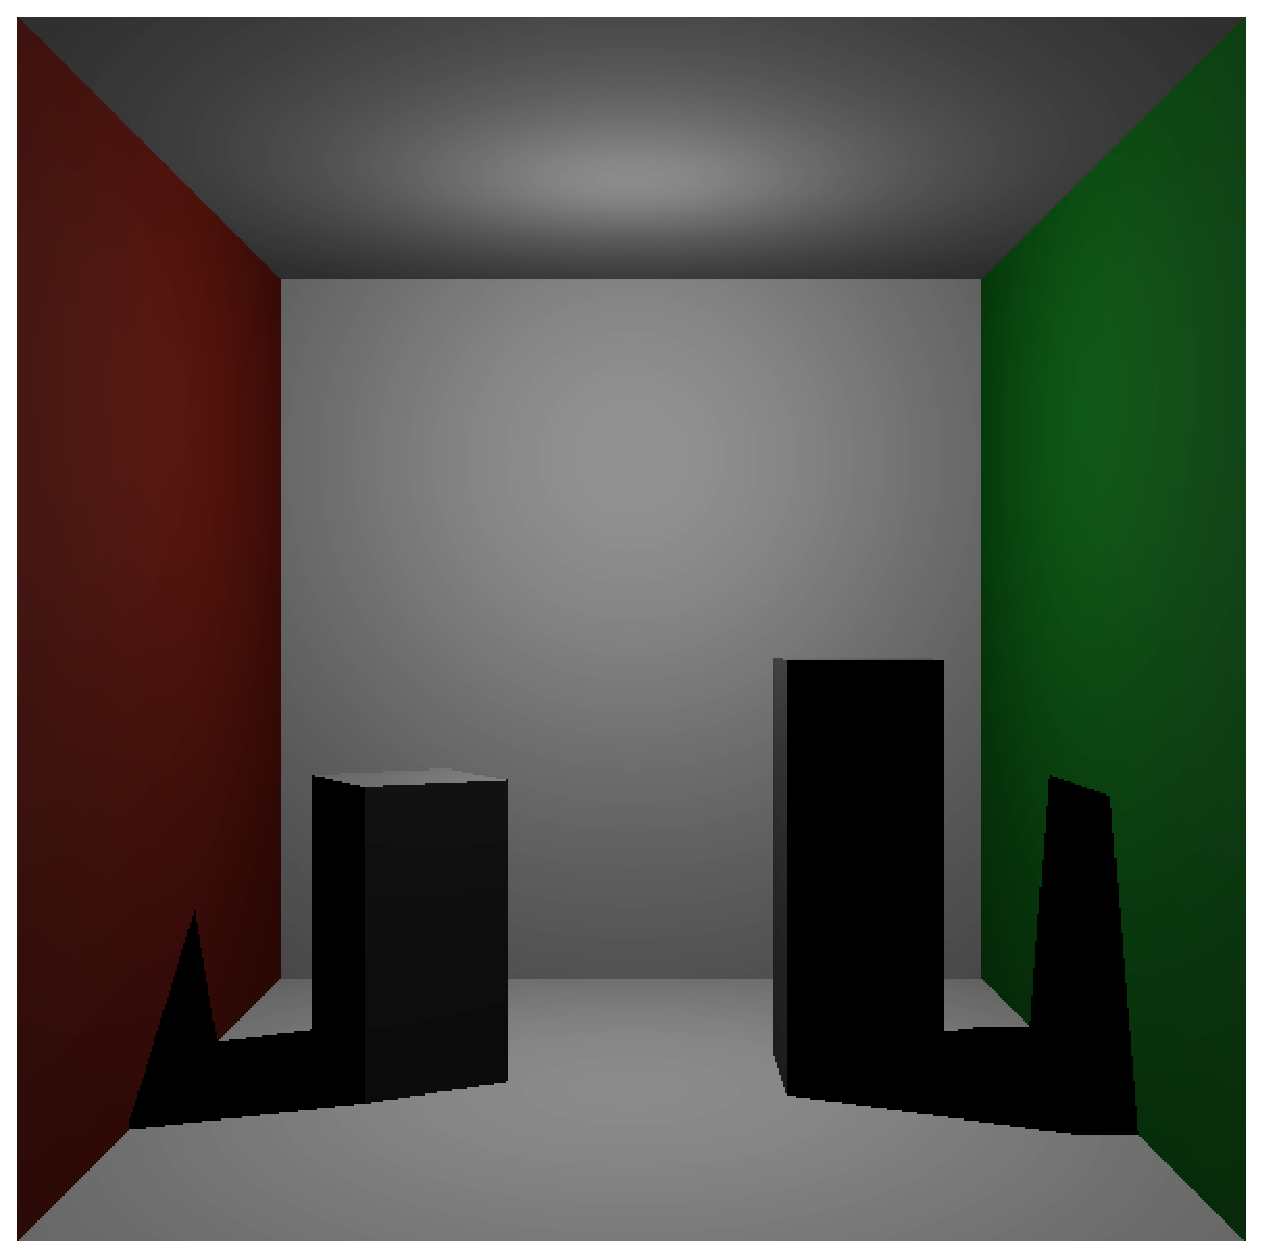
\includegraphics[width=\textwidth]{../img/boxes_noindirect}
        \end{column}
    \end{columns}

\end{frame}




\subsection{Global Illumination}
%%--------------------------------------------  BACKGROUND: GLOBAL ILLIMUNATION
\begin{frame}{Global Illumination}

    \begin{columns}
        \begin{column}{0.65\textwidth}
            Definition of global illumination\\
            Graphics and Light\\

        \end{column}
        \begin{column}{0.35\textwidth}
            %%\rput[lb](0,0){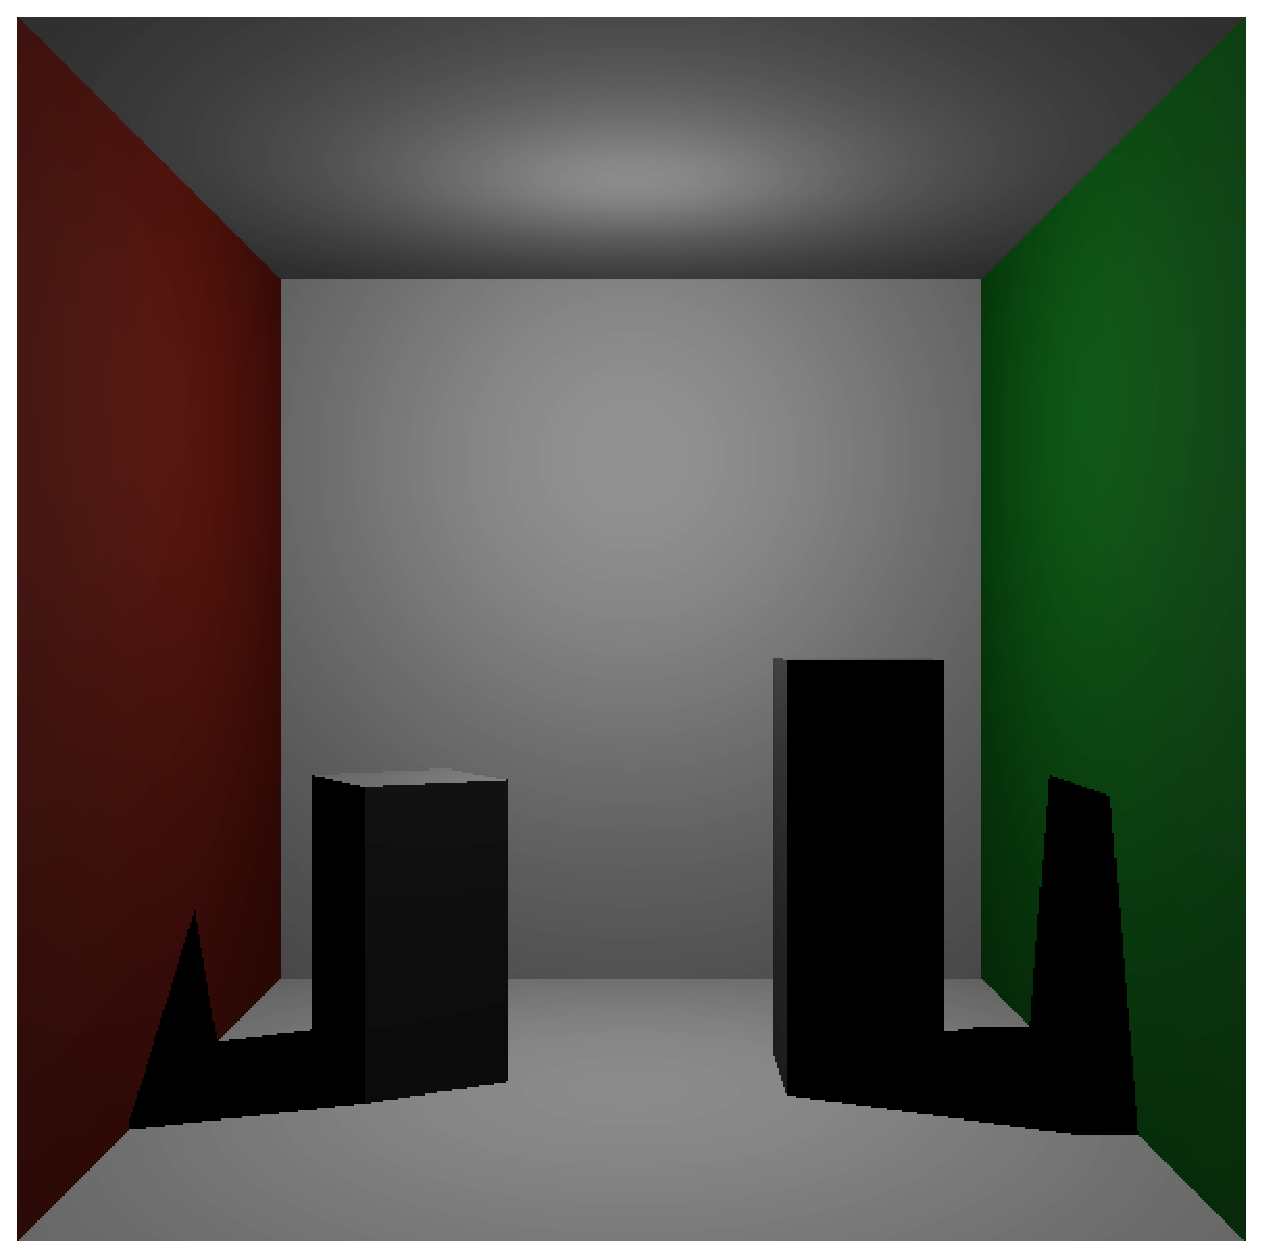
\includegraphics[width=\textwidth]{../img/boxes_noindirect}}
            %%\rput[lt](0,0){\includegraphics[width=\textwidth]{../img/indirect_box_high}}
            \vspace{0mm}
            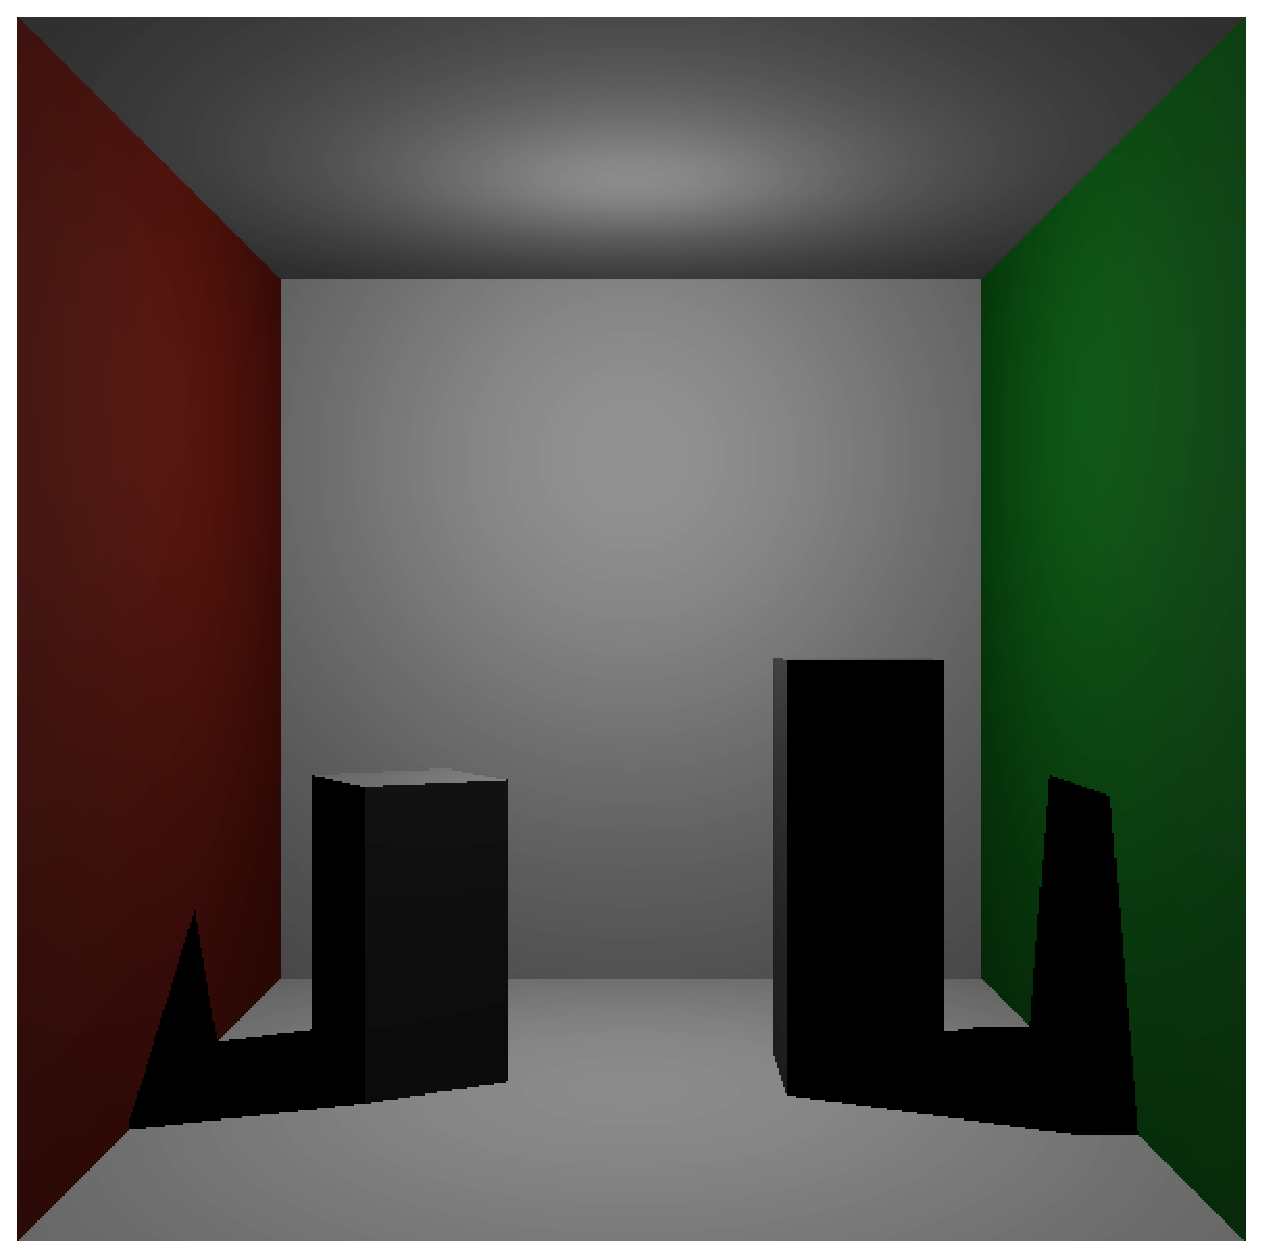
\includegraphics[width=\textwidth]{../img/boxes_noindirect}
            \vspace{2mm}
            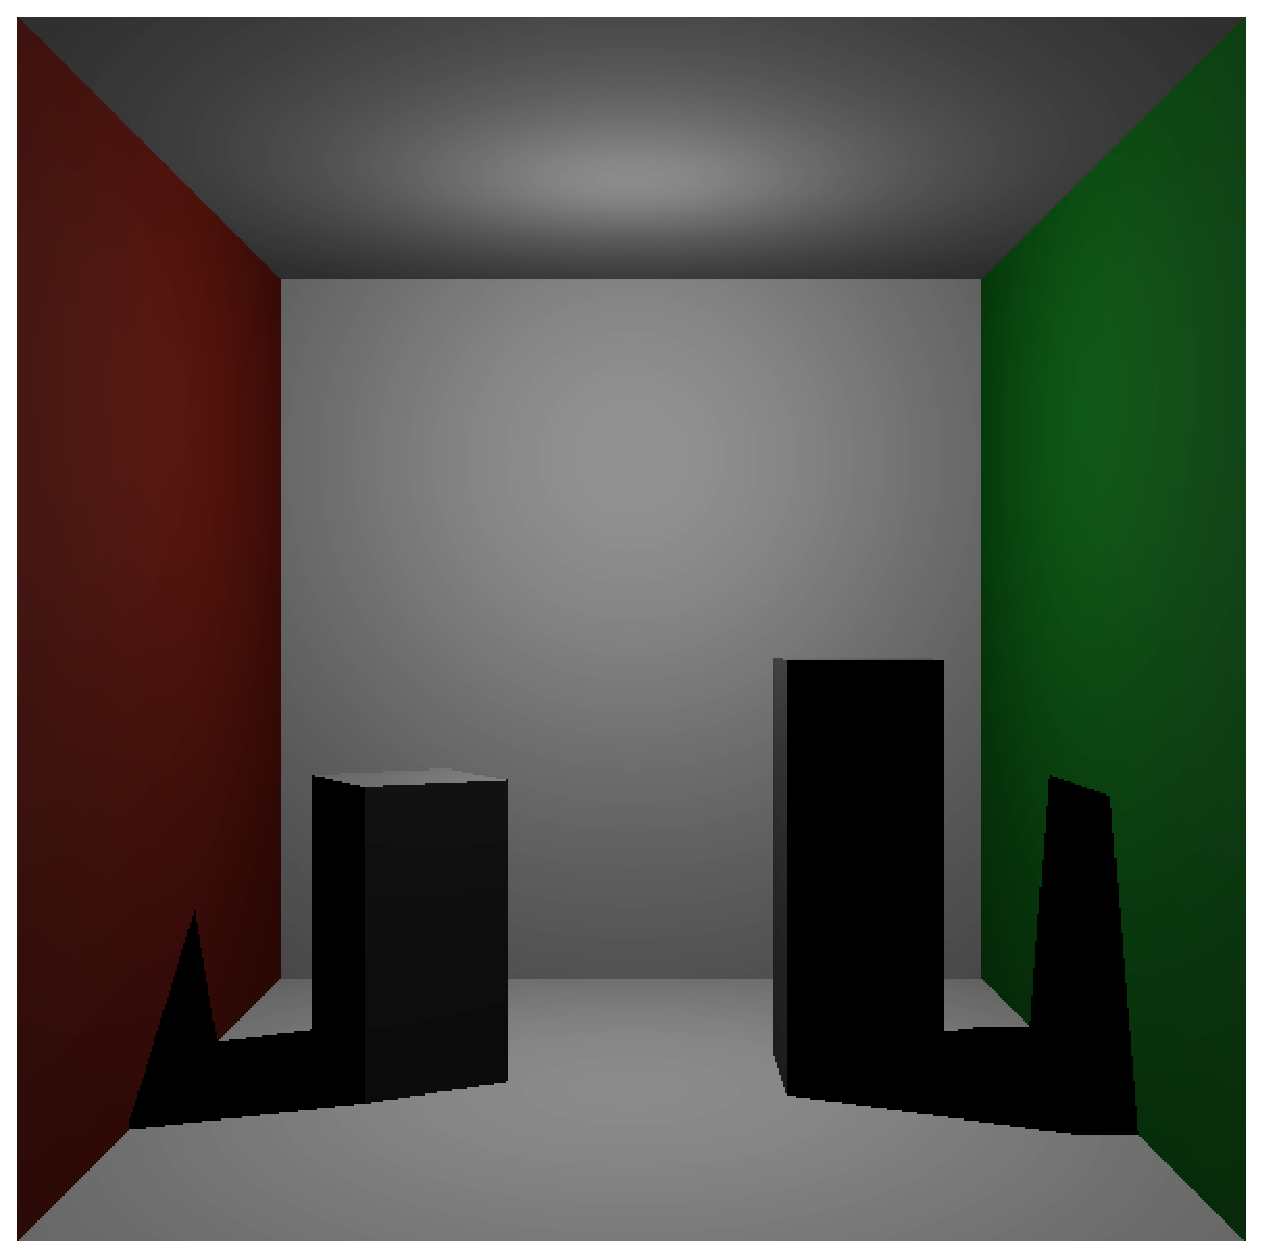
\includegraphics[width=\textwidth]{../img/boxes_noindirect}
        \end{column}
    \end{columns}

\end{frame}




\subsection{Point-Based Color Bleeding}
%%------------------------------------------------  BACKGROUND: VOLUME LIGHTING
\begin{frame}{Point-Based Color Bleeding}

Cheap, accurate global illumination effects using color bleeding
Utilizes direct light point cloud representation of scene

\end{frame}




\subsection{Problem Statement}
%%------------------------------------------  RELATED WORK: GLOBAL ILLIMUNATION
\begin{frame}{Problem Statement}

Most GA algorithms do not include volume contributions

\end{frame}




\subsection{Our Contribution}
%%------------------------------------------  RELATED WORK: GLOBAL ILLIMUNATION
\begin{frame}{Our Contribution}

Modification to PCB to allow GA effects in scenes with volumes
Allows for render speedups of a factor of ten.

\end{frame}




\section{Background}
\subsection{Graphics Background}
%%-----------------------------------------------------------------  BACKGROUND
\subsection{Illumination and Light}
%%---------------------------------------------------  BACKGROUND: ILLIMUNATION
\begin{frame}{Flux and Radiance}

    \begin{block}{Flux}
        The measure of total light emitted. 
    \end{block}  

    \begin{block}{Radiance}
        \[
        \mathit{L} = \frac{\mathit{d^{2}\Phi}}{\mathit{dw\:dA}^\perp}.
        \]

        % NOTE: Flux density per unit area, per unit solid angle
        % NOTE: dA is the projection of dA on a plane perpendicular to w
        % NOTE: radiance is incoming light power

    \end{block}

\end{frame}




%%---------------------------------------------------  BACKGROUND: ILLIMUNATION
\begin{frame}{Flux and Radiance}

    

    \begin{block}{Radiance Invariance}
        \[
            L(x \to y) = L(y \to x).
        \]
    \end{block}

\end{frame}




%%---------------------------------------------------  BACKGROUND: ILLIMUNATION
\begin{frame}{Irradiance}

    \begin{block}{Irradiance}
        Measure of {\em emitted} light
        \[
            E = \frac{d\Phi}{dA}
        \]

        %NOTE: Flux density per area
        %NOTE: Counts as "emitted radiance"
    \end{block}

    Consider irradiance due to surrounding radiance...

    \begin{block}{Irradiance}
        \[
            \mathit{E} = \int\mathit{L}(\textup{p} \leftarrow w)\textup{cos}\theta dw.
        \]
    \end{block}

\end{frame}




%%---------------------------------------------------  BACKGROUND: ILLIMUNATION
\begin{frame}{Irradiance}

    \centering
    \vspace{-1cm}
    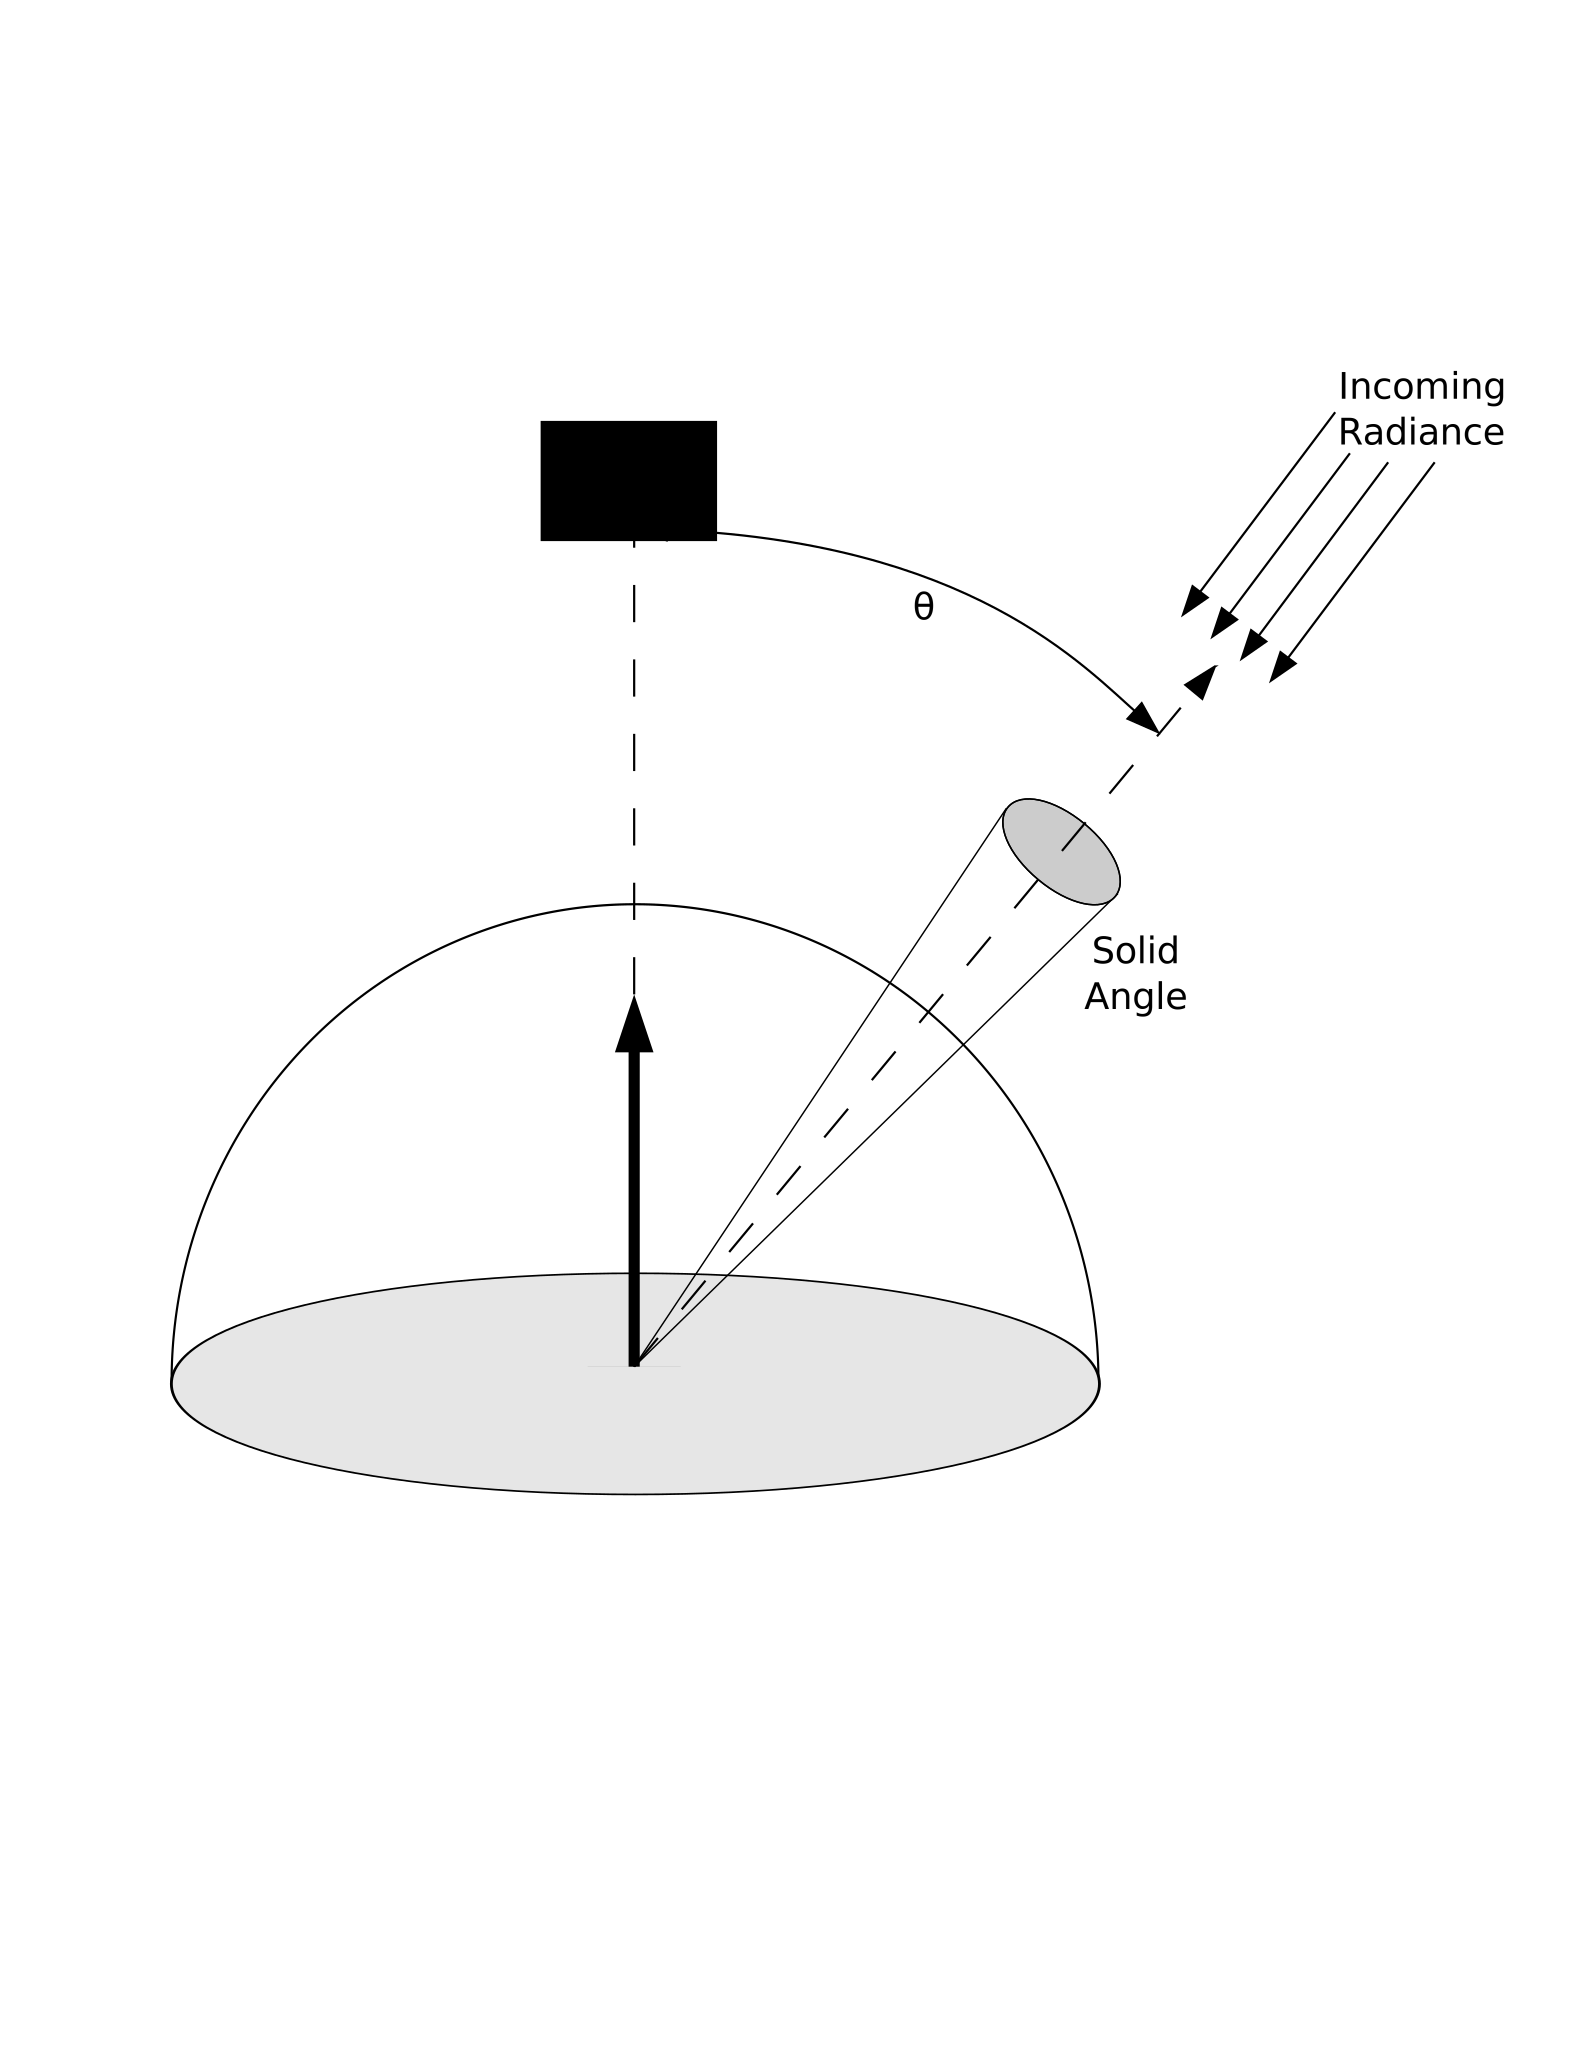
\includegraphics[height=80mm]{../img/diag/radiance.pdf}

\end{frame}




\subsection{BRDF}
%%-----------------------------------------------------------  BACKGROUND: BRDF
\begin{frame}{BRDF}

    \begin{center}
        {\bf B}idirectional {\bf R}eflectance {\bf D}istribution {\bf F}unction
    \end{center}

    Gives us a formalism for describing the reflection from a surface

    Helps evaluate irradiance leaving the surface towards the viewer.

    Recall:

    \begin{block}{Differential Irradiance}
        \[
            \mathit{dE}(\textup{p}, w_i) = \int\mathit{L_i}(\textup{p} \leftarrow w_i)\textup{cos}\theta_i dw_i.
        \]
    \end{block}
    

\end{frame}




\subsection{BSRDF}
%%---------------------------------------------------  BACKGROUND: ILLIMUNATION
\begin{frame}{BSRDF}

    \begin{center}
        {\bf B}idirectional {\bf S}cattering-surface {\bf R}eflectance {\bf D}istribution {\bf F}unction
    \end{center}

    Describes complex behavior of light within surface (\emph{subsurface scattering}.)

    Describes ratio of exitant light based on incoming light and outgoing direction.

    Exponentially more complex.

\end{frame}




\subsection{Volume Lighting}
%%---------------------------------------------------  BACKGROUND: ILLIMUNATION
\begin{frame}{Volume Lighting}

    \centering
    \vspace{0cm}
    
\includegraphics[width=100mm]{../img/diag/vol_scatter.pdf}

\end{frame}




\subsection{Volume Lighting}
%%---------------------------------------------------  BACKGROUND: ILLIMUNATION
\begin{frame}{Volume Lighting}

    \begin{block}{Absorption}
        \[
            e^{-\int_{0}^{d}\sigma_{a} (p+t\mathit{w},\mathit{w})d\mathit{t}}.
        \]
    \end{block}

    \begin{block}{Scatter Out}
        \[
            \textup{d}\mathit{L}_{o}(\textup{p},w) = -\sigma_{s}(\textup{p},w) \mathit{L}_{i}(\textup{p},-w)\textup{d}t.
        \]
    \end{block}

\end{frame}




%%---------------------------------------------------  BACKGROUND: ILLIMUNATION
\begin{frame}{Volume Lighting}

    \centering
    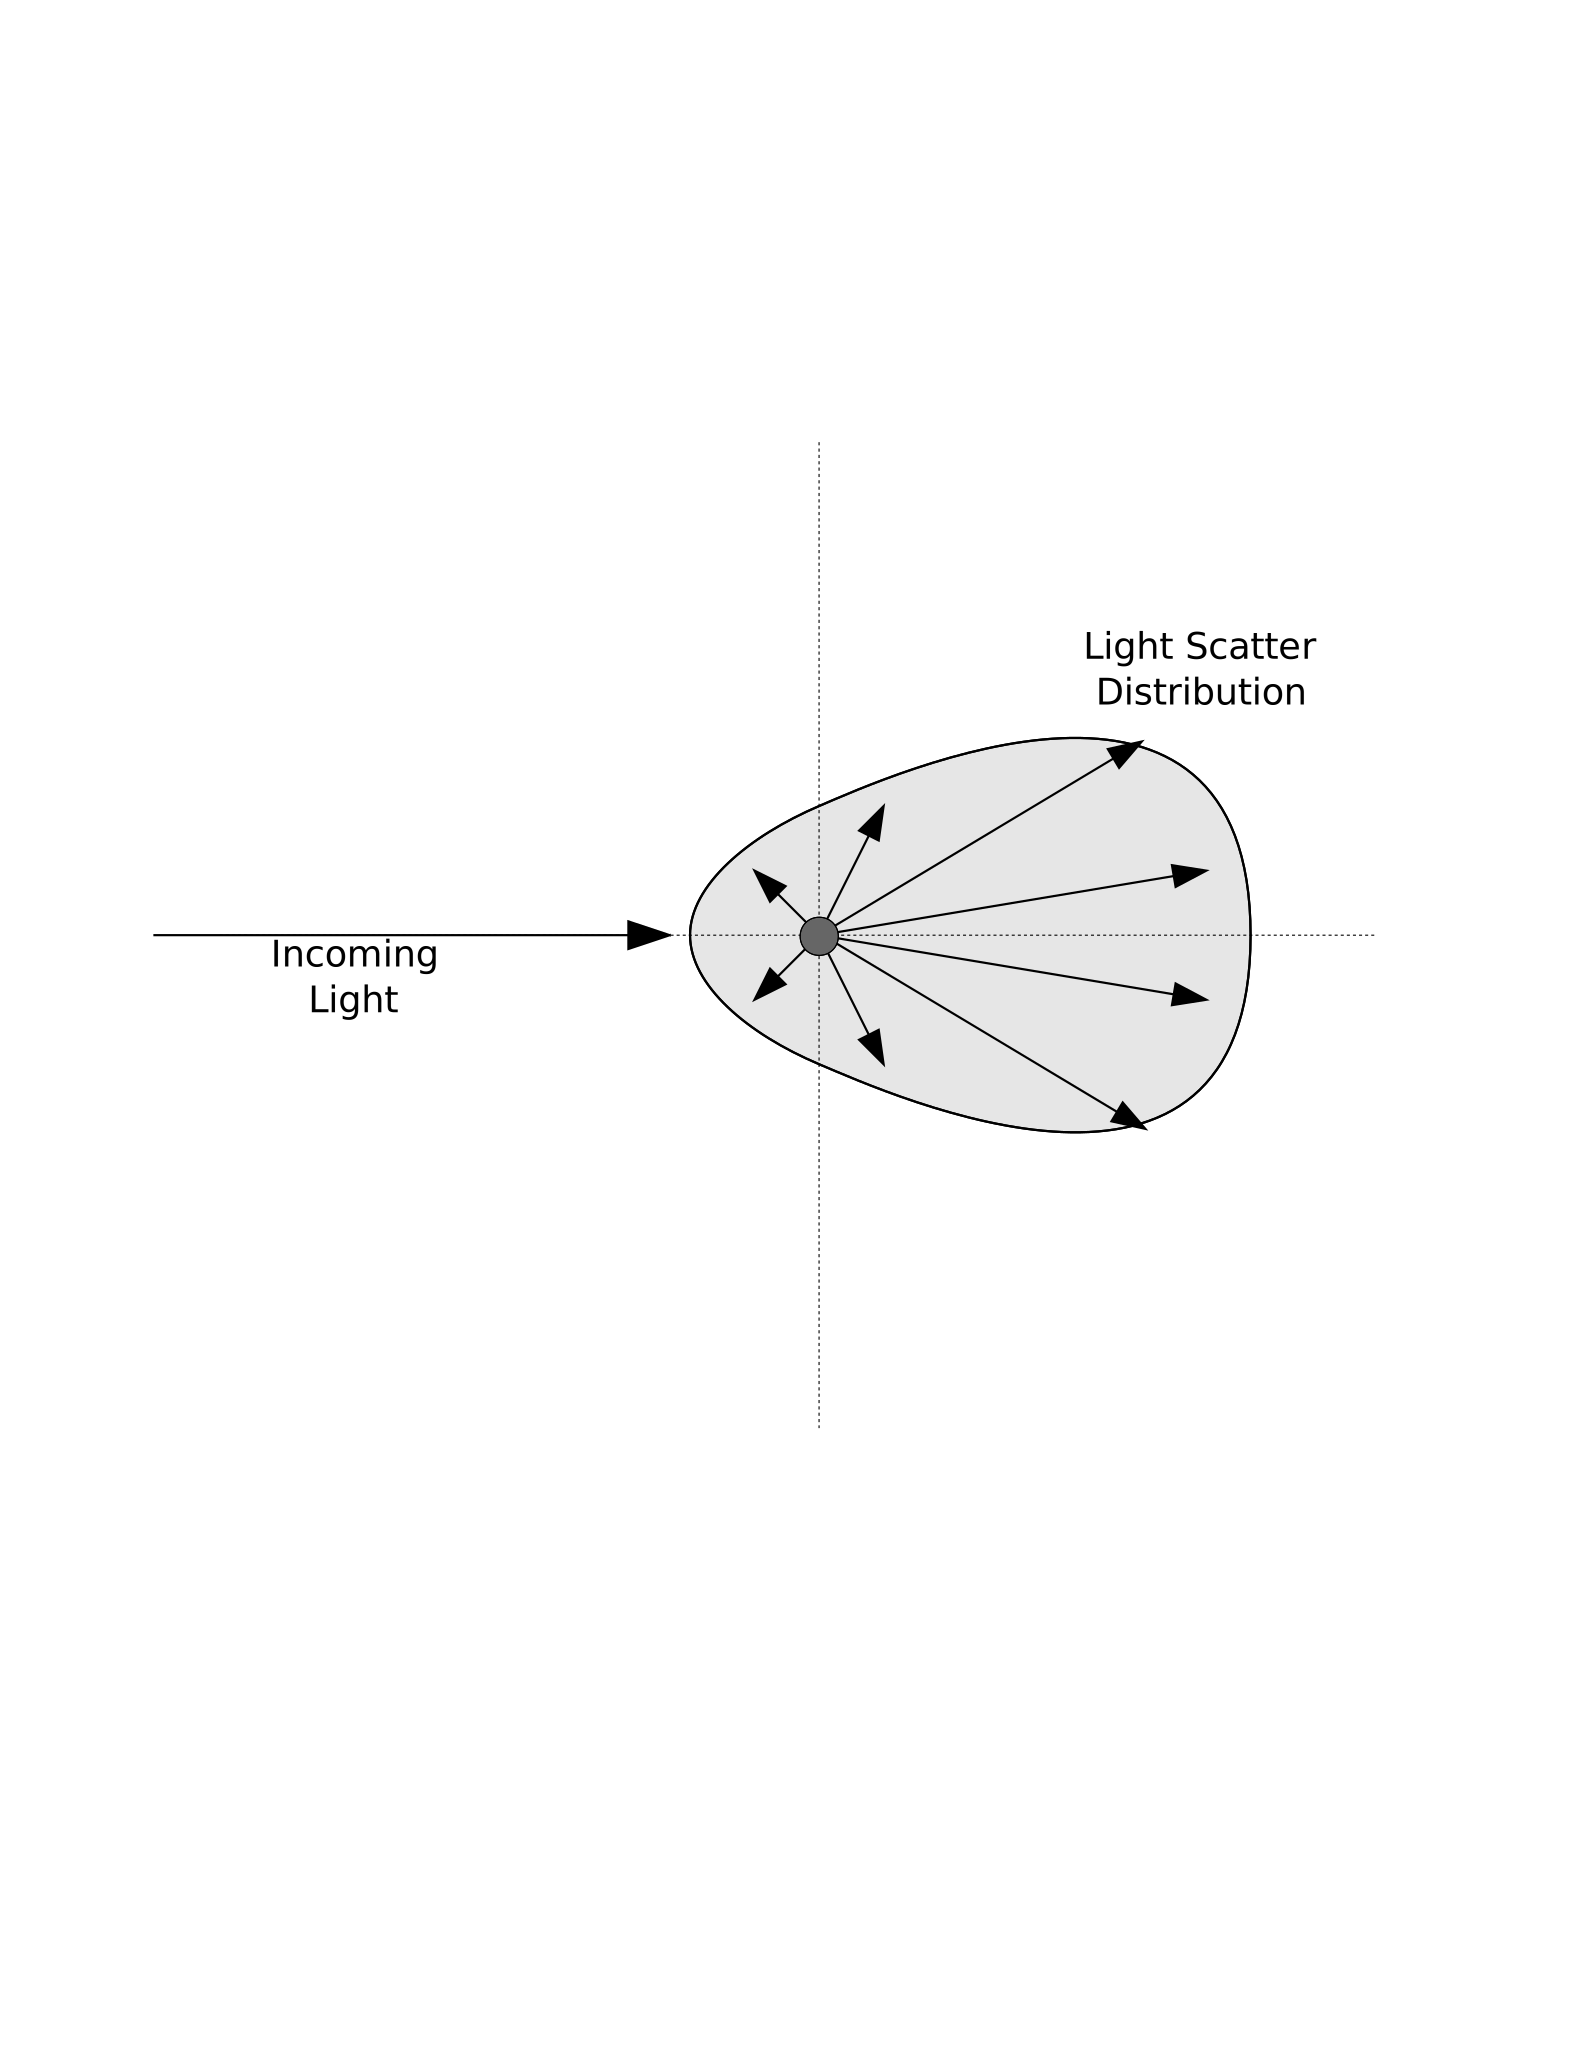
\includegraphics[width=80mm]{../img/diag/phase_func}

\end{frame}




%%---------------------------------------------------  BACKGROUND: ILLIMUNATION
\begin{frame}{Volume Lighting}

    \begin{block}{Phase Function}
        Described as $phase(w \to w')$
    \end{block}

    \begin{block}{Source Normalization}
        \[
            \int_{\mathbb{S}^2}phase(w \to w')\textup{d}w' = 1.
        \]
    \end{block}

\end{frame}




%%---------------------------------------------------  BACKGROUND: ILLIMUNATION
\begin{frame}{Volume Lighting}

    \begin{block}{Transmittance}
        \[
            T_{r}(\textup{p} \to \textup{p}') = e^{-\int_{0}^{d}\sigma (p+t\mathit{w},\mathit{w})d\mathit{t}}.
        \]
    \end{block}

    \begin{block}{Scatter In}
        \[
            \mathit{S}(\textup{p},w) = \mathit{L}_{\textup{ve}}(\textup{p},w) + \sigma_{\textup{s}}(\textup{p}, w) \int_{\mathbb{S}^2} phase(\textup{p}, -w' \to w) L_{i}(\textup{p},w')\textup{d}w'.
        \]
    \end{block}

\end{frame}




\subsection{Monte Carlo Integration}
%%-----------------------------------------------  BACKGROUND WORK: MONTE CARLO
\begin{frame}{Monte Carlo Integration}

    Monte Carlo methods allow estimation of complex systems through use of probability functions and random numbers.

    Most useful is Monte Carlo Integration.

    Allows random, discrete sampling of a function.

    Allows estimation of an arbitrary integral.

\end{frame}




\section{Related Work}
\subsection{Global Illumination}
%%------------------------------------------  RELATED WORK: GLOBAL ILLIMUNATION
\begin{frame}{Related Works: Global Illumination}

    Field of study in computer graphics.

    Photon Mapping.

    Radiosity.

    Monte Carlo Techniques.

\end{frame}




%%------------------------------------------  RELATED WORK: GLOBAL ILLIMUNATION
\begin{frame}{Related Works: Point-Based Color Bleeding}

    Point-Based Approximate Color Bleeding by Per Christensen.

    Subset of scene geometry is thoroughly sampled, creating point cloud.

    Point cloud is sampled to determin incoming radiance.

\end{frame}




%%------------------------------------------  RELATED WORK: GLOBAL ILLIMUNATION
\begin{frame}{Related Works: Photon Mapping}

    \includegraphics[width=100mm]{../img/external/ewr7_mcbox.jpg}

\end{frame}




\subsection{Volume Rendering}
%%---------------------------------------------  RELATED WORK: VOLUME RENDERING
\begin{frame}{Related Works: Volume Rendering}

    A number of approaches...

    Polygonal representation based on isosurfaces

    Opacity/Color arrays (interpolation across voxels)

\end{frame}




%%---------------------------------------------  RELATED WORK: VOLUME RENDERING
\begin{frame}{Related Works: Volume Rendering}

    Multi-Resolution Volumes

    Occlusion Techniques

\end{frame}




%%---------------------------------------------  RELATED WORK: VOLUME RENDERING
\begin{frame}{Related Works: Volume Rendering}

    Volume Lighting

\end{frame}




\section{PCB Extension Algorithm}
\subsection{Point-Based Color Bleeding}
%%--------------------------------------------------------------  PCB EXTENSION
\begin{frame}{Point-Based Color Bleeding}

    \begin{enumerate}
        \item Sample the scene and generate a point cloud
        \item Perform ray tracing on regular geometry
        \item Replace ambient estimates with a gather stage using surrounding point cloud
    \end{enumerate}

\end{frame}




\subsection{Extension Overview}
%%--------------------------------------------------------------  PCB EXTENSION
\begin{frame}{Extension Overview}

    \begin{enumerate}
        \item Sample the scene and generate a point cloud
        \item Sample the participating media and evaluate scatter, absorbtion and direct lighting
        \item Cast rays as normal
        \item Orient hemispherical samples along the normals of the surfaces intersected
        \item Model scatter-out and scatter-in properties during lighting gather stage
    \end{enumerate}

\end{frame}




\subsection{Sampling the Scene}
%%--------------------------------------------------------------  PCB EXTENSION
\begin{frame}{Sampling the Scene}

    \centering
    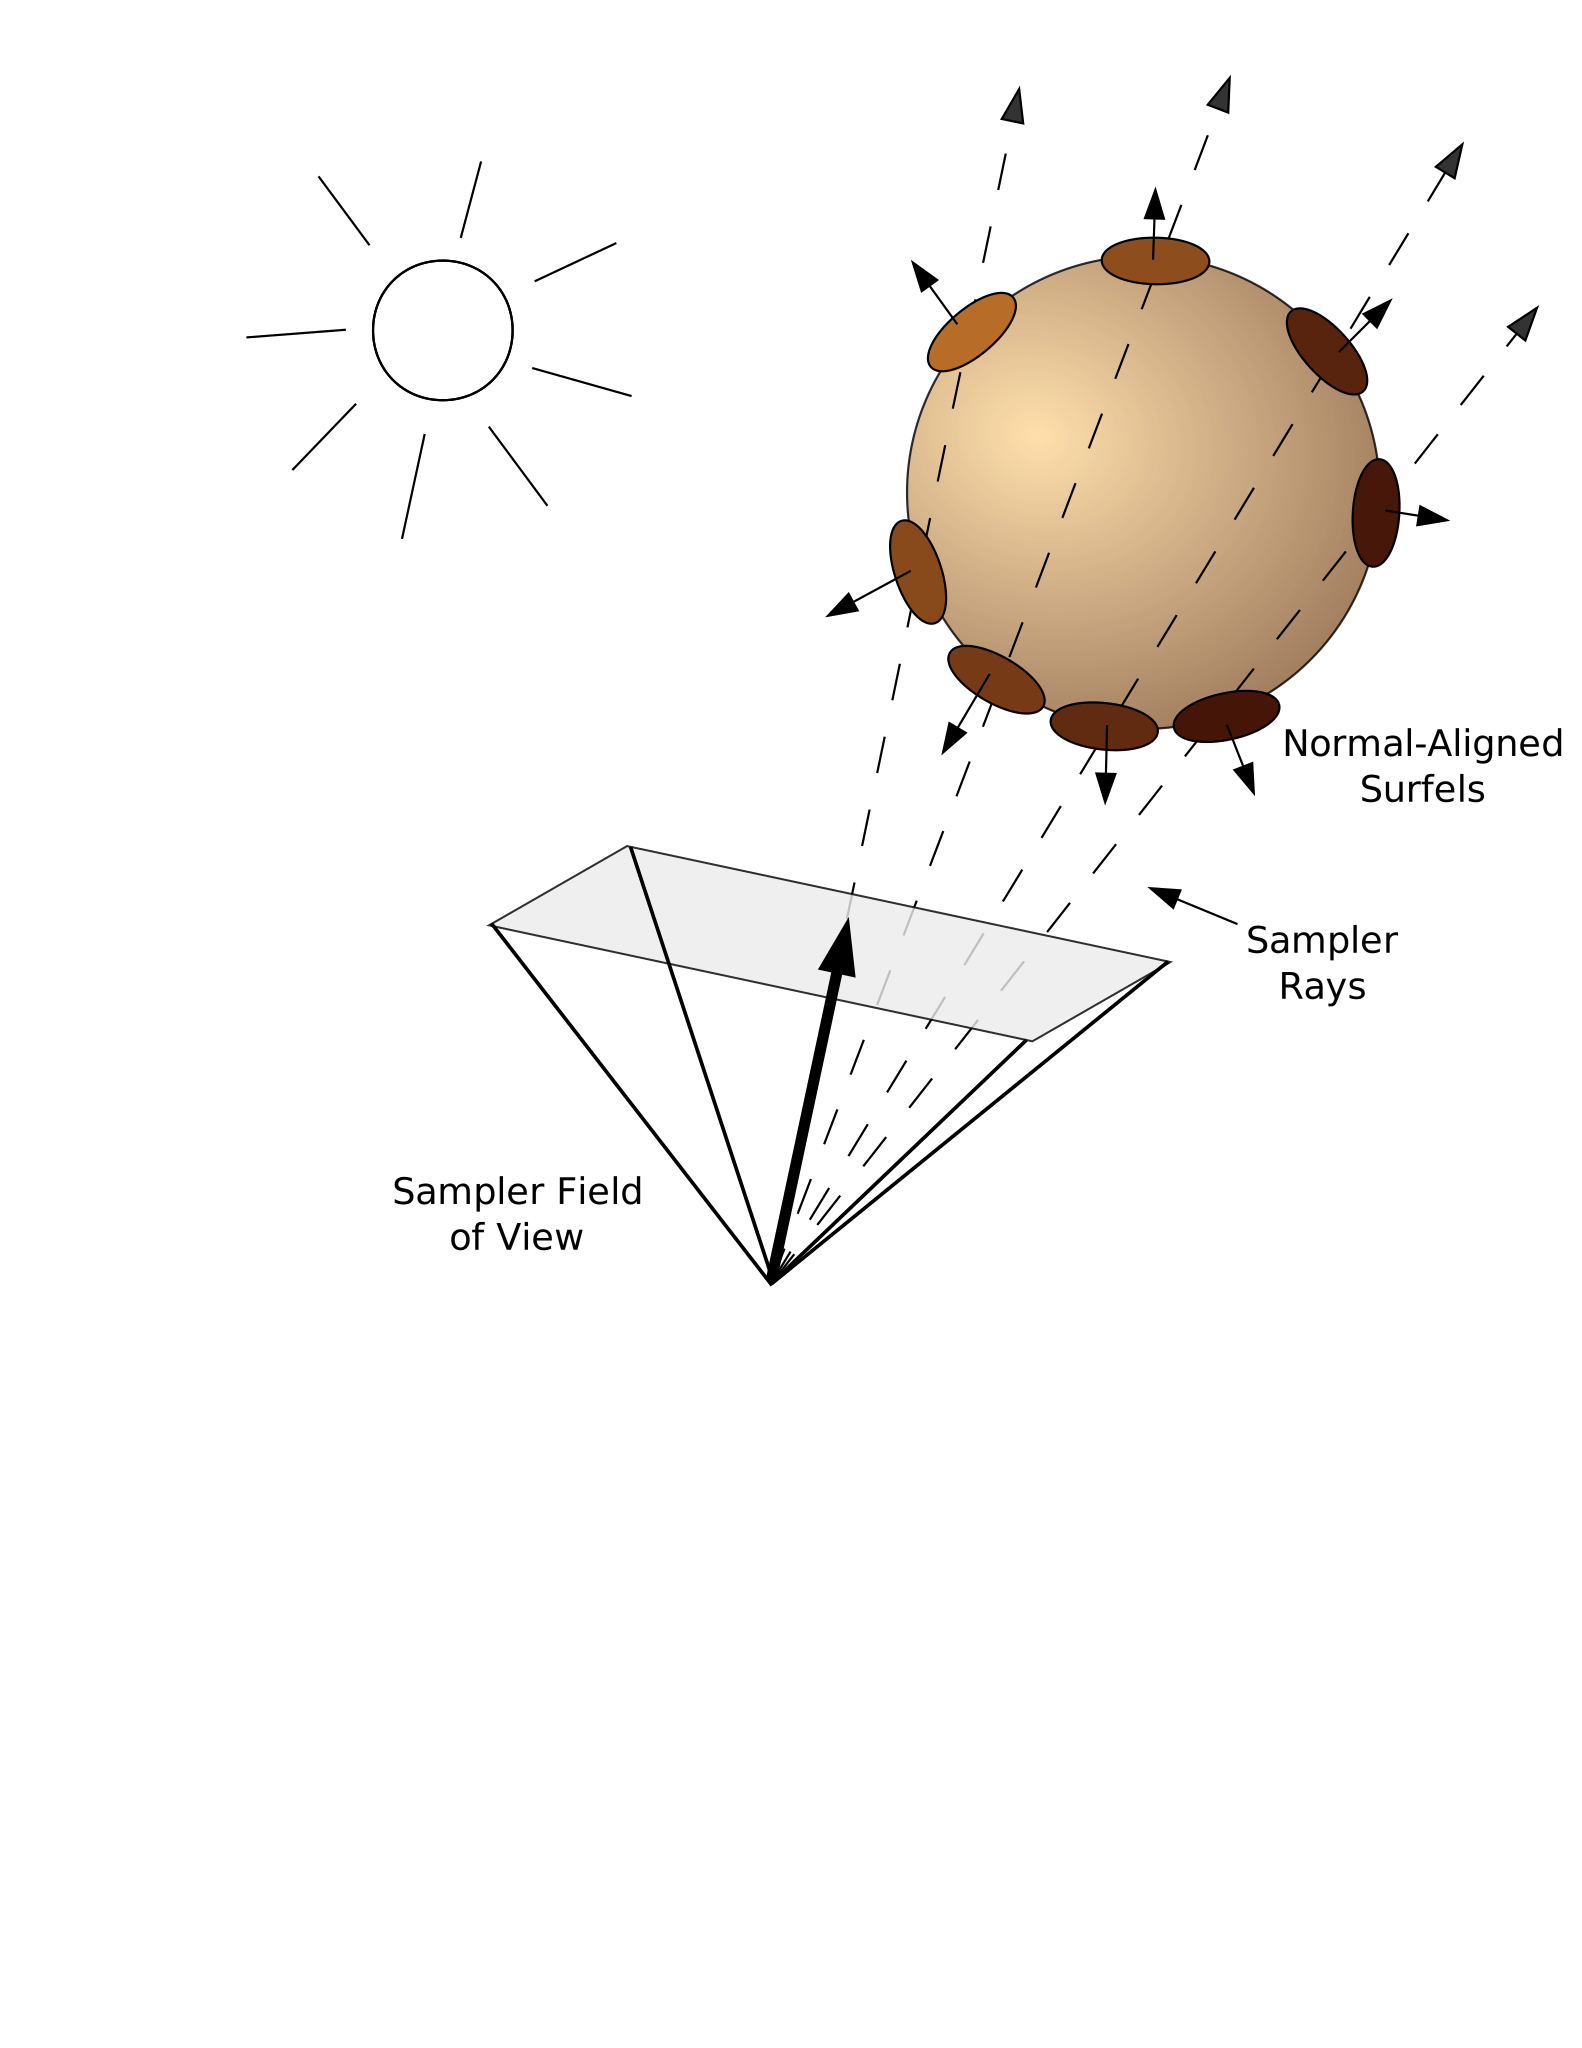
\includegraphics[height=70mm]{../img/diag/surfel_samp.pdf}

\end{frame}




\subsection{Gathering Light}
%%--------------------------------------------------------------  PCB EXTENSION
\begin{frame}{Gathering Light}

    \centering
    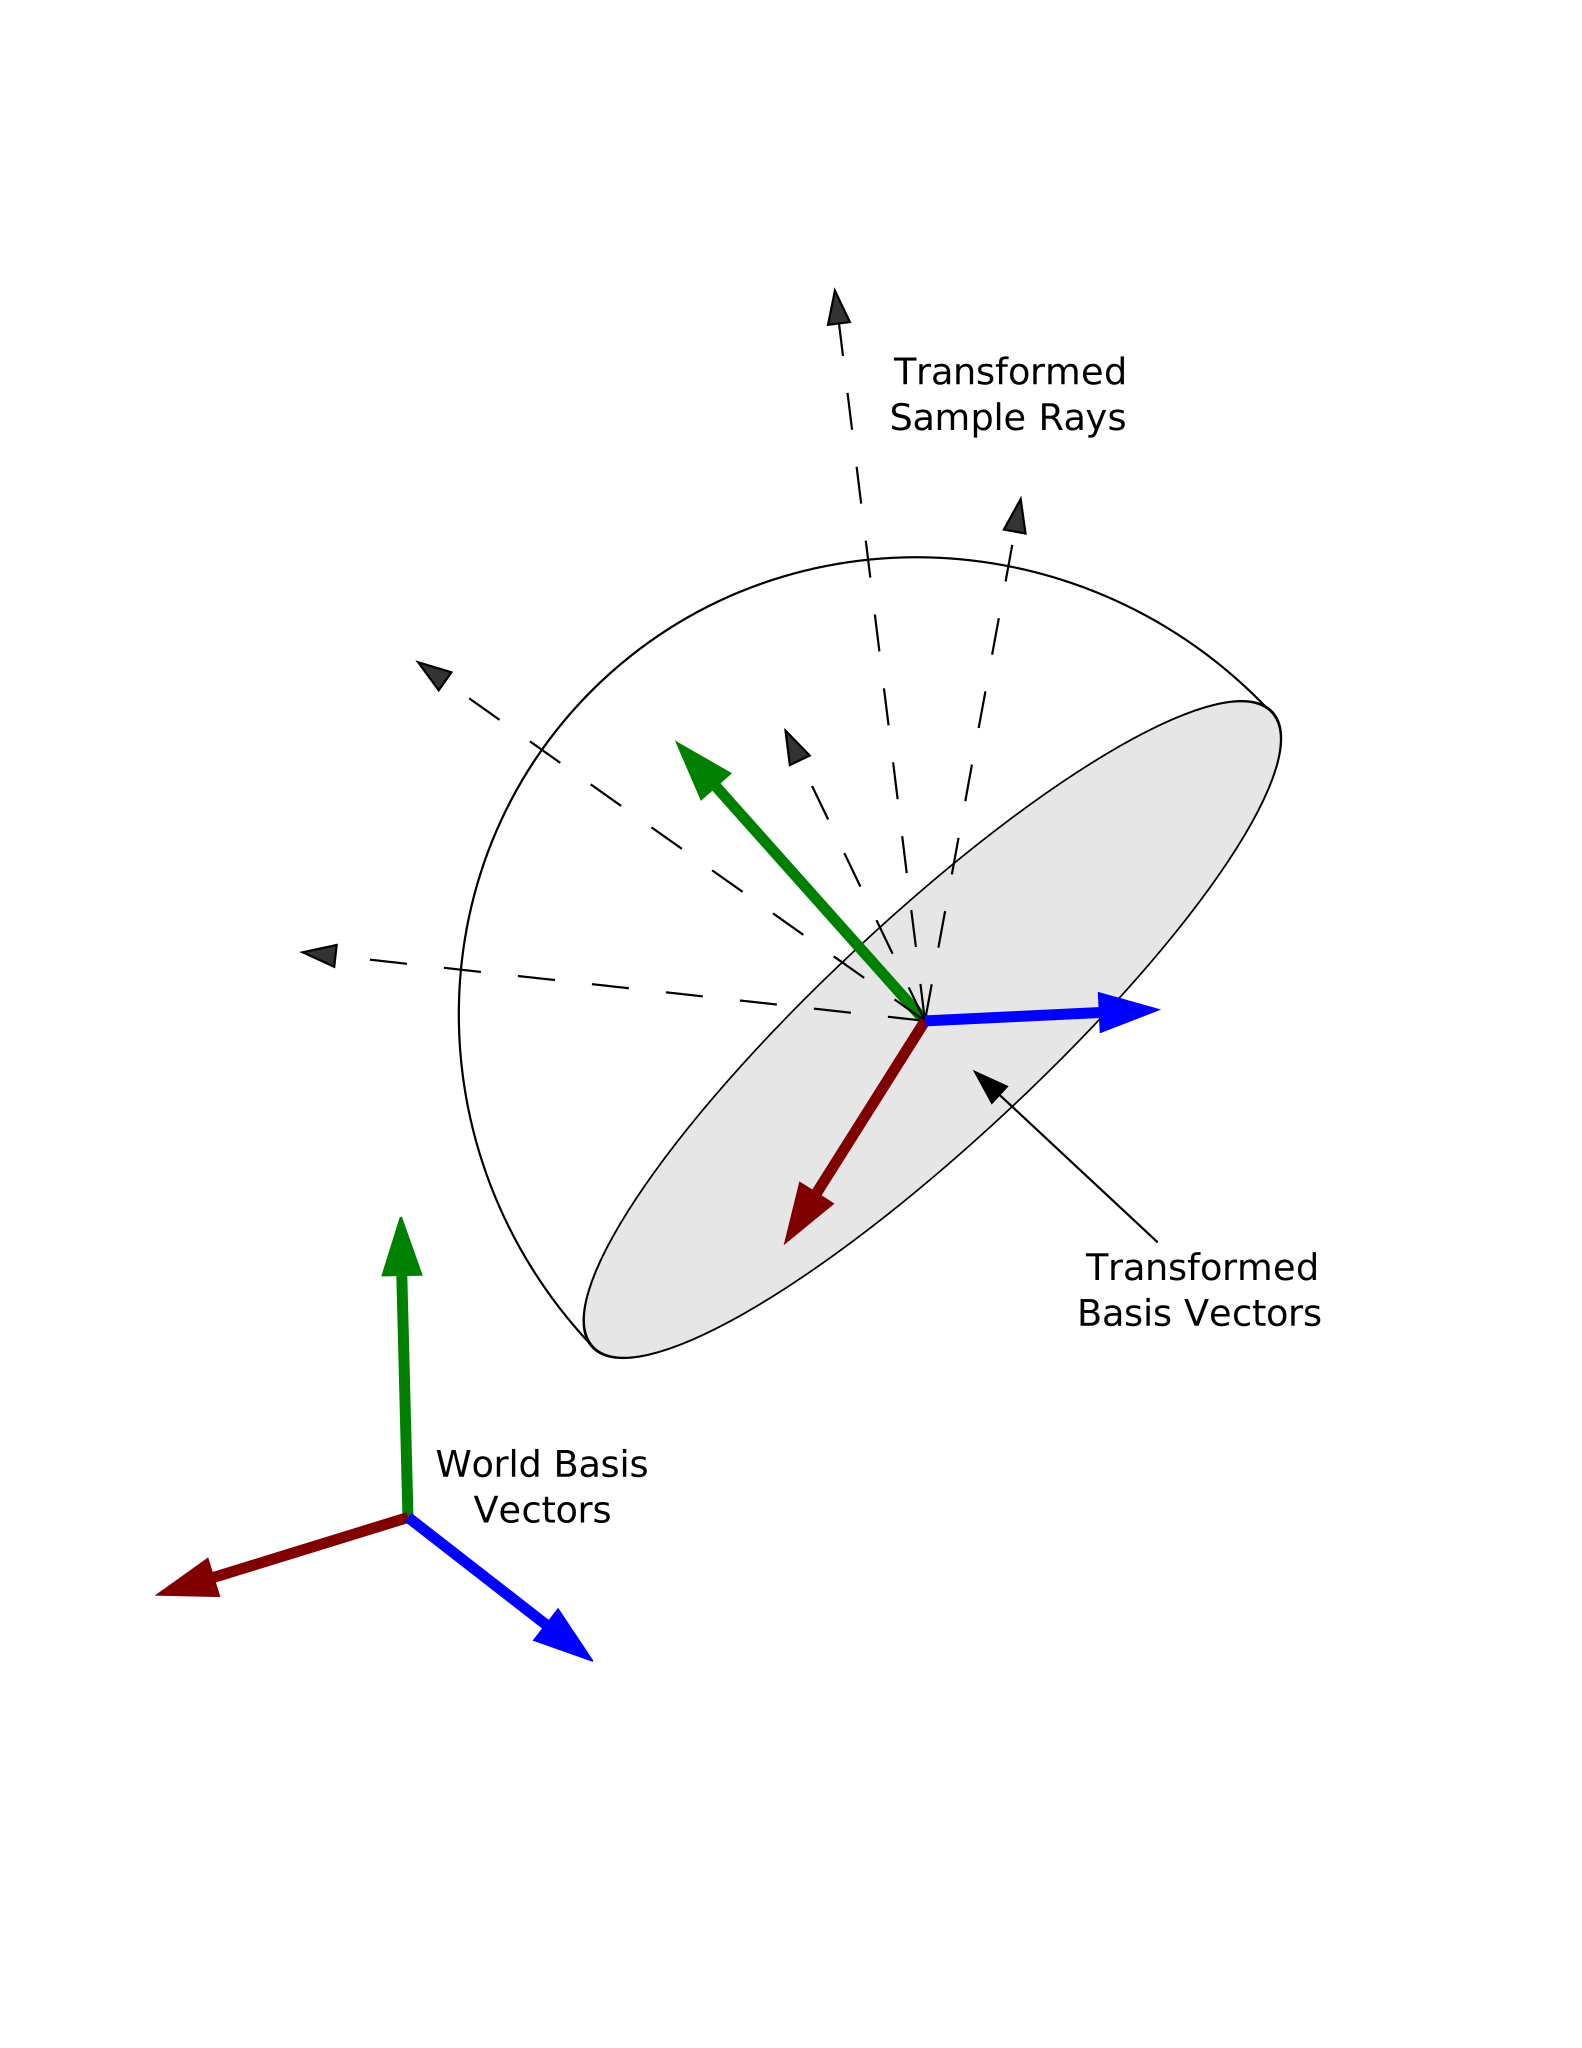
\includegraphics[height=70mm]{../img/diag/orthnormal.pdf}

\end{frame}




\subsection{Gathering Light}
%%--------------------------------------------------------------  PCB EXTENSION
\begin{frame}{Gathering Light}

    \centering
    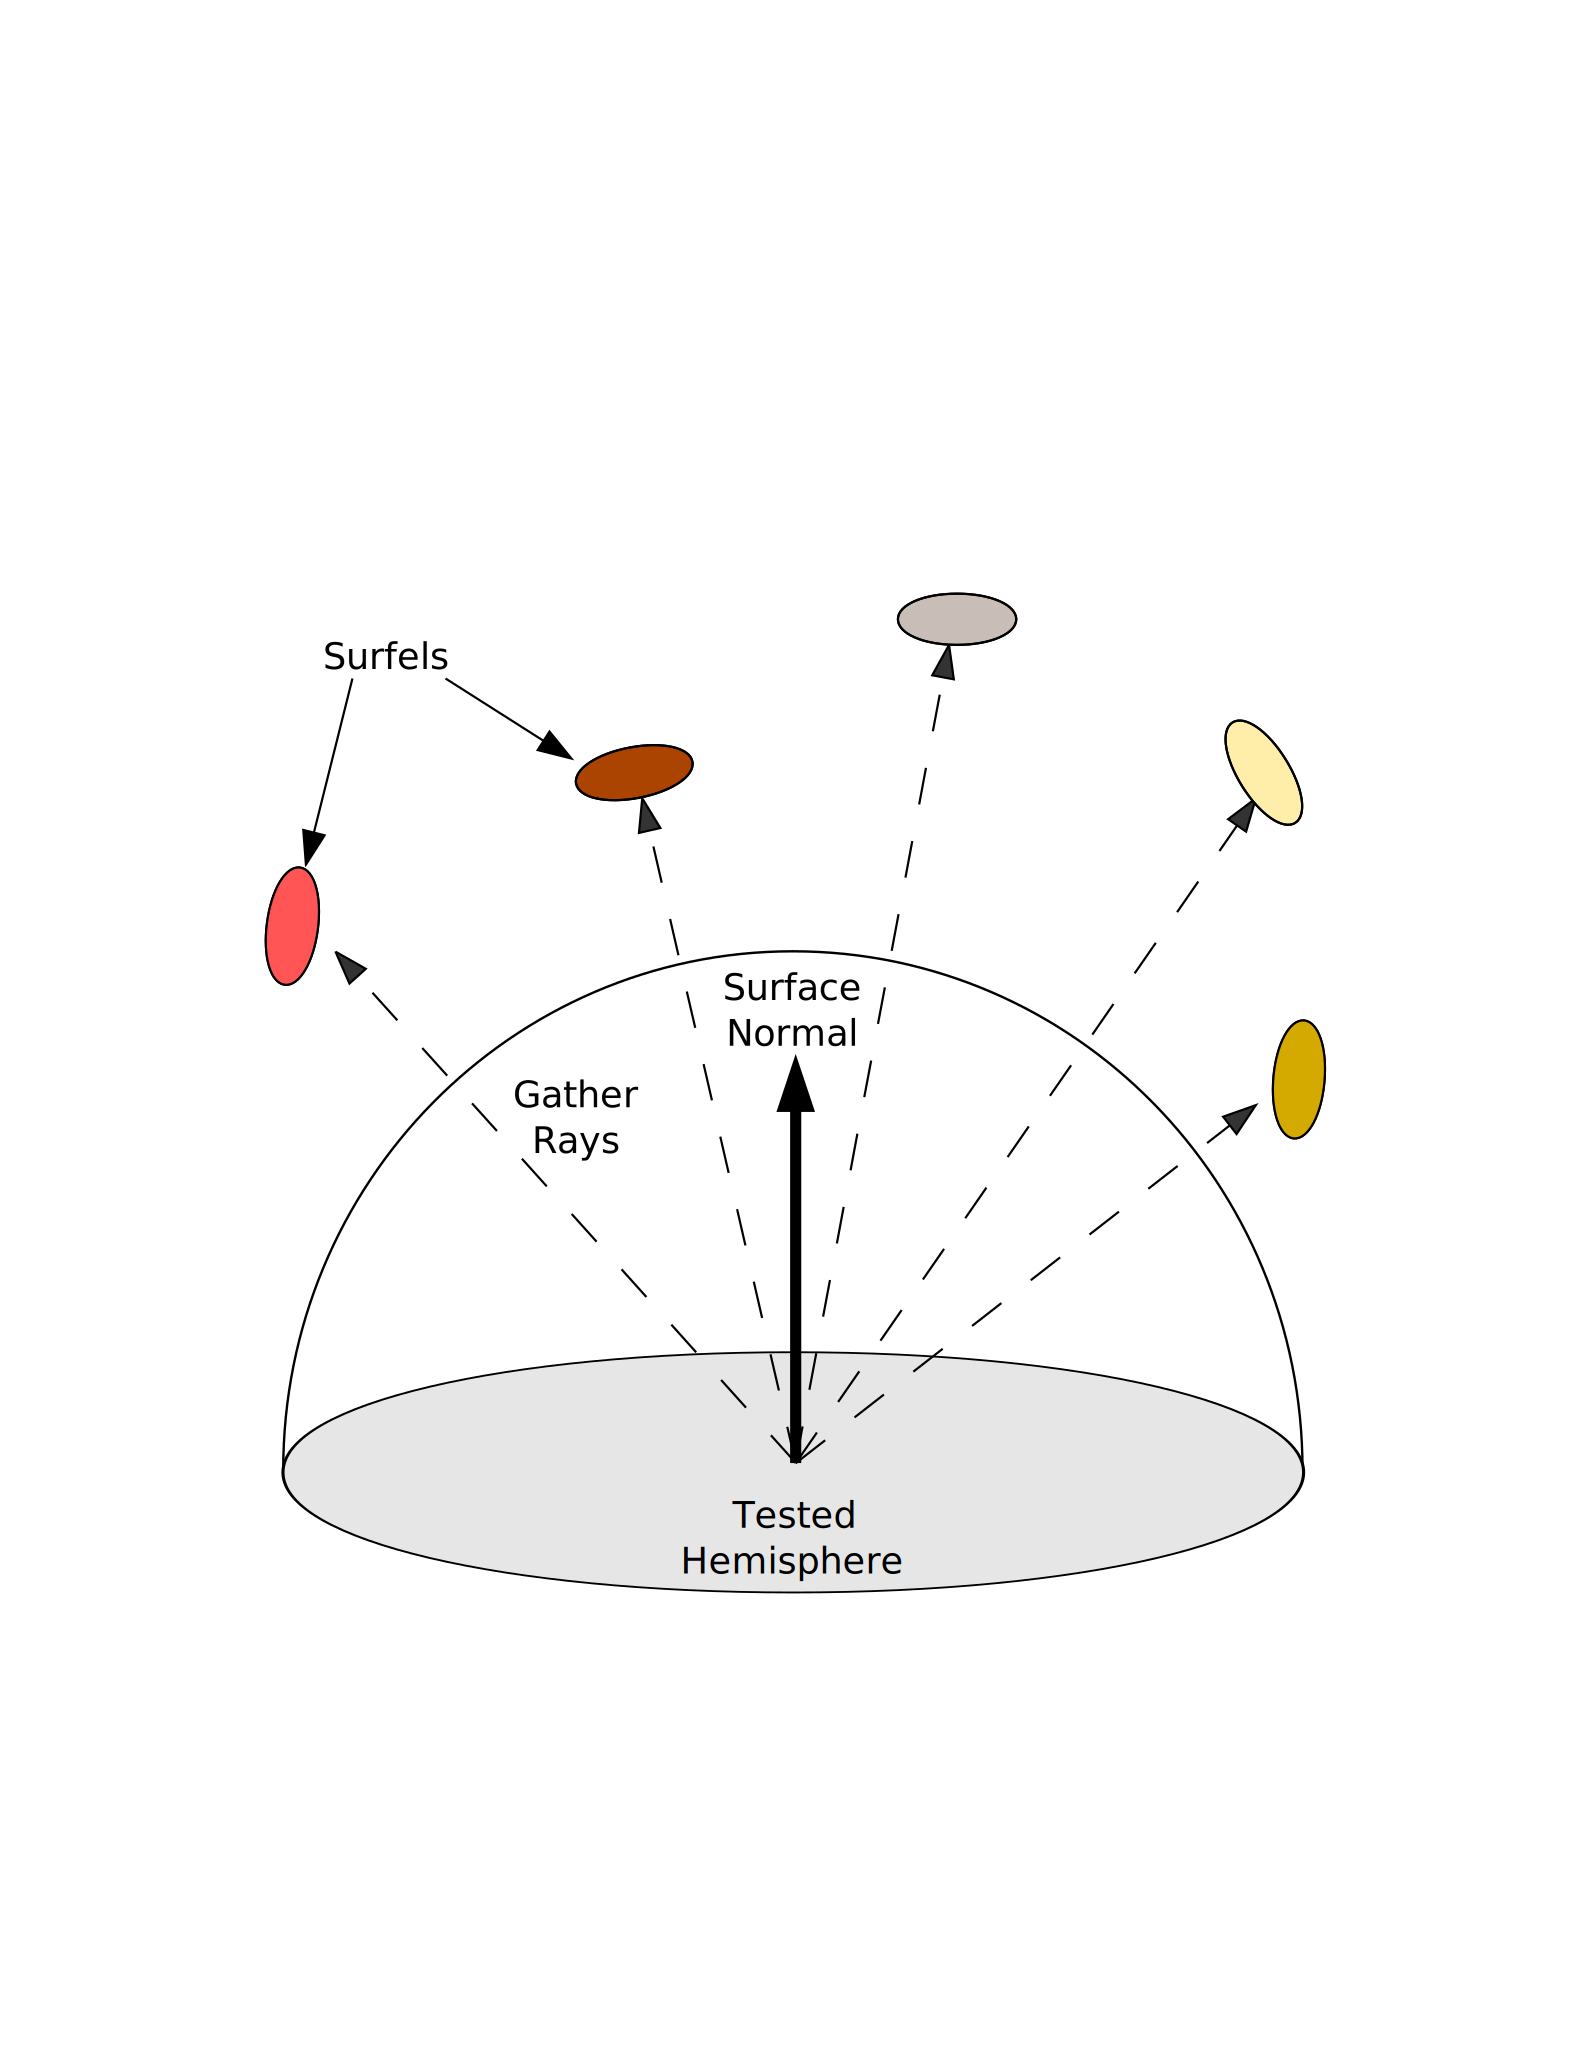
\includegraphics[height=70mm]{../img/diag/gather.pdf}

\end{frame}




\subsection{Integrating Volume Data}
%%--------------------------------------------------------------  PCB EXTENSION
\begin{frame}{Integrating Volume Data}

    \centering
    \includegraphics[height=70mm]{../img/testing.png}

\end{frame}




\section{Results}
%%--------------------------------------------------------------------  RESULTS
\begin{frame}{Results}

    \begin{center}
    \setlength{\tabcolsep}{5pt}
    \begin{tabular}{ | l | c | c | c | }
      \hline                       
      Scene & Render Time (s) & Image Delta & Memory Overhead \\
      \hline                  
      Monte Carlo w/o PCB & 3351 sec & NONE & NONE \\
      Traditional PCB & 348 sec & 11.0\% & 390 Mb (4.0\%) \\
      Extended PCB & 397 sec & 4.8\% & 395 Mb (4.1\%)  \\
      \hline  
    \end{tabular}
    \end{center}

\end{frame}




\section{Future Work}
%%--------------------------------------------------------------------  RESULTS
\begin{frame}{Future Work}

    \begin{enumerate}
        \item Multiple bounce
        \item Phase functions for volumes
        \item Parallelism
        \item Optimal Sampling
        \item GPU Acceleration
    \end{enumerate}

\end{frame}




\section{Conclusion}
%%-----------------------------------------------------------------  CONCLUSION
\begin{frame}{Conclusion}

    Oh yea!

\end{frame}

\end{document}
